\documentclass[12pt]{amsart}
\usepackage{tikz}
\usetikzlibrary {shapes.geometric}
\title{Activity 1}
\begin{document}
\begin{enumerate}
\item Write down the sequence that are formed by pentagons. Find the pattern in this sequence and see if the same can be done for other geometric objects.
\begin{figure}
    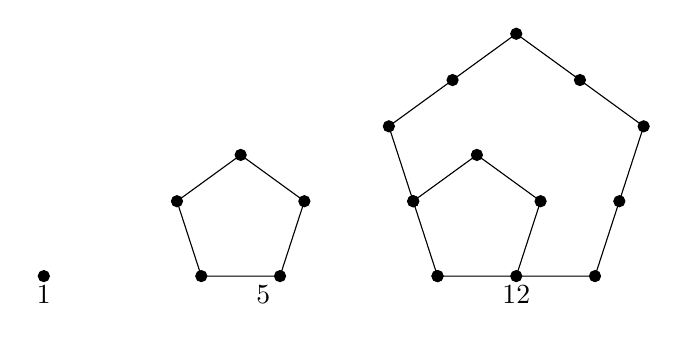
\begin{tikzpicture}
        \filldraw (0,0) node[below]{$1$} circle [radius=2pt];
        \filldraw (2,0) circle [radius=2pt] --++ (0:1)node[below left]{$5$} circle [radius=2pt] --++ (72:1) circle [radius=2pt] --++ (144:1) circle [radius=2pt] --++ (216:1) circle [radius=2pt] --++ (288:1) circle [radius=2pt];
        \filldraw (5,0) circle [radius=2pt] --++ (0:1) circle [radius=2pt] --++ (72:1) circle [radius=2pt] --++ (144:1) circle [radius=2pt] --++ (216:1) circle [radius=2pt] --++ (288:1) circle [radius=2pt];
        \filldraw (5,0) circle [radius=2pt] ++ (0:1)node[below]{$12$} --++ (0:1) circle [radius=2pt] --++ (72:1) circle [radius=2pt] --++ (72:1) circle [radius=2pt] --++ (144:1) circle [radius=2pt] --++ (144:1) circle [radius=2pt] --++ (216:1) circle [radius=2pt] --++ (216:1) circle [radius=2pt] --++ (288:1) circle [radius=2pt];

      \end{tikzpicture} 
\end{figure}

% \item (MCQ) Which is larger? Twice the sum of the first $1000$ natural numbers, or the sum of the first $1000$ odd natural numbers?
%   \begin{enumerate}
%   \item Twice the sum of the first $1000$ natural numbers.
%   \item the sum of the first $1000$ odd natural numbers.
%   \item They are equal.
%   \end{enumerate}
%   Correct answer: (b).
% \item (Short answer) Find a formula for $1+4+7+\dotsb+3n-2$ (the sum of first $n$ numbers which leave remainder $1$ when divided by $3$.
%   \\
%   Correct answer: $(3n-1)n/2$.
% \item (MSQ) Which following is the same as
%   \begin{displaymath}
%     \sum_{i=1}^n \sum_{j=1}^i (2i+j)
%   \end{displaymath}
%   for all positive integers $n$?
%   \begin{enumerate}
%   \item $$\sum_{i=1}^n \sum_{j=1}^i (2j+i)$$
%   \item $$\sum_{j=1}^n \sum_{i=j}^n (2i+j)$$
%   \item $$\sum_{j=1}^n \sum_{i=1}^j (2i+j)$$
%   \item $$\sum_{i=1}^n \sum_{j=i}^n (2j+i)$$
%   \end{enumerate}
%   Correct answers: (b) and (d).
% \item (Short Answer) The \emph{Online Encyclopedia of Integer Sequences (OEIS)} (https://oeis.org) has a huge collection of integer sequences.
%   Each sequence has a unique identifier.
%   For example, the sequence of triangular numbers has identifier A000217 and can be found at https://oeis.org/A000217.
%   Consider the sequence $\{C_n\}$ given by the rule:
%   \begin{itemize}
%   \item $C_0=1$.
%   \item $C_n = \sum_{k=0}^{n-1} C_k C_{n-1-k}$ for $n\geq 1$.
%   \end{itemize}
%   What is the unique identifier of this sequence on OEIS?

%   Correct Answer: A000108
% \item (Numerical, exact value) Use OEIS to find $C_{30}$ in the previous problem
  
%   Correct answer: 3814986502092304
% \item (MCQ) Let $S_n = \{x\in \mathbf N\mid x \text{ is divisible by } n\}$.
%   Then $S_9\cap S_{12}$ is equal to which of the following sets?
%   \begin{enumerate}
%   \item $S_{72}$
%   \item $S_3$
%   \item $S_{36}$
%   \item $S_{24}$
%   \end{enumerate}
%   Correct answer: (c).
% \item Let $S_n$ be as in the previous problem.
%   How many natural numbers less than 100 are elements of $S_9\cup S_{12}$?
%   \begin{enumerate}
%   \item $3$
%   \item $17$
%   \item $19$
%   \item $33$
%   \end{enumerate}
\end{enumerate}
\end{document}
